\documentclass[a4paper,openright,twoside,11pt]{report}

%% Define margins
\usepackage[top=5.35cm,bottom=5.35cm,left=4cm,right=4cm]{geometry}


%% Spacing in paragraphs
\parindent12pt
\parskip6pt

%% The "usual" math packages
\usepackage{amsfonts}
\usepackage{amsmath}
\usepackage{amssymb}

% The Greek language, indentation and keyboard
\usepackage{indentfirst}
\usepackage[english,greek]{babel}
\usepackage[iso-8859-7]{inputenc}

% Type \en{text} for latin alphabet
\newcommand{\en}{\latintext}

% Some fun with figures
\usepackage{graphicx}

\usepackage{fancyhdr}

\renewcommand{\headrulewidth}{0pt}


%% Define shortcuts
\newcommand{\uoiauthor}{Όνομα Επίθετο}
\newcommand{\uoiyear}{2013}
\newcommand{\uoititle}{\LARGE\textsc{Τίτλος Διατριβής}}
\newcommand{\examdate}{Ημερομηνία εξέτασης}

\newcommand{\thesisdedication}{Αφιερώνεται στον/στην ...}

\newcommand{\advisor}{Όνομα Επίθετο}
\newcommand{\rankadvisor}{Καθηγητής}
%
\newcommand{\examinera}{Όνομα Επίθετο}
\newcommand{\ranka}{Αναπληρωτής Καθηγητής}
%
\newcommand{\examinerb}{Όνομα Επίθετο}
\newcommand{\rankb}{Επίκουρος Καθηγητής}
%
\newcommand{\examinerc}{Όνομα Επίθετο}
\newcommand{\rankc}{Καθηγητής}
%
\newcommand{\examinerd}{Όνομα Επίθετο}
\newcommand{\rankd}{Αναπληρωτής Καθηγητής}
%
\newcommand{\examinere}{Όνομα Επίθετο}
\newcommand{\ranke}{Επίκουρος Καθηγητής}
%
\newcommand{\examinerf}{Όνομα Επίθετο}
\newcommand{\rankf}{Καθηγητής}

\usepackage[Sonny]{fncychap_uoi}

\begin{document}
\ChTitleVar{\Huge\sc}
%%%%%%%%%%%%%%%%%%%%%%%%%%%%%%%%%%%%%%%%%%%%%%%%%%%%%%%%%%%%%%%%
%% Use abstract.tex for the abstract in Greek and abstract_english.tex for
%% the abstract in english. Should you need to thank anyone (like your advisor!)
%% use the ackno.tex file.
%% Do not edit the lines below!
\thispagestyle{empty}

\noindent\begin{tabular}{l c r}
{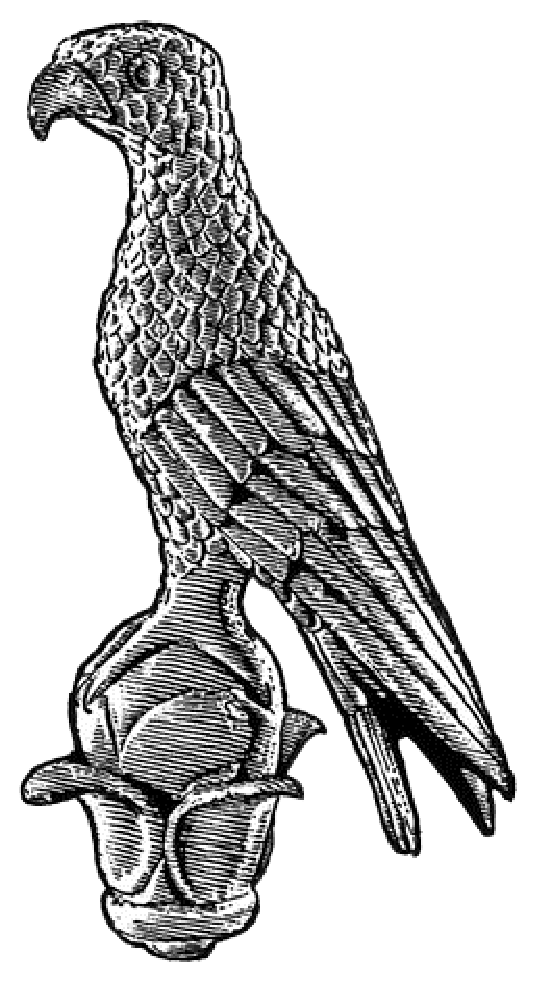
\includegraphics[width=1.3cm]{eagle.eps}} & \raisebox{4.7\height}
{\bf \Large ������������ ���������} & %\raisebox{.15\height}
{\hfill
\includegraphics[width=2.46cm]{math_logo.eps}}\\[-1.3cm]
& {\textsc{\textbf{\LARGE ����� �����������}}}
\end{tabular}

\vspace*{\stretch{.3}}

\begin{center}
{\Large\bf\uoiauthor}
\end{center}

\vspace*{\stretch{.2}}

\noindent\rule{\linewidth}{0.5mm}
%
\begin{center}
\uoititle
\end{center}
%
\noindent\rule{\linewidth}{0.5mm}

\vspace*{\stretch{.3}}

\begin{center}
{\Large ������������ ��������}
\end{center}



\vspace*{\fill}

\begin{center}
{\Large ��������, \uoiyear}
\end{center}

\newpage\thispagestyle{empty}\mbox{}\newpage


\thispagestyle{empty}

\vspace*{0.1\paperheight}

\begin{flushright}
{\em \thesisdedication}
\end{flushright}

\newpage\thispagestyle{empty}\mbox{}\newpage

\thispagestyle{empty}
\thispagestyle{empty}
\parindent0pt

� ������� ������������ �������� ���������� ��� ������� ��� ������� ��� ���
�������� ��� ������������� ���������� ���������� ���/���..... ��� �������� �� ����� ����������� ���
������������� ���������.

\vskip1cm

��������� ��� ..../..../.....   ��� ��� ���������� ��������: \bigskip

\begin{tabular}{ll}

  {\bf �������������} & {\bf �������}  \\[12pt]
   \advisor  & \rankadvisor   \\[12pt]
   \examinera & \ranka \\[12pt]
   \examinerb & \rankb \\[12pt]


\end{tabular}

\vskip2cm



\vfill

\begin{center} �������� ������
\end{center}

{\en ``}������ �������� ��� � ������� �������� ���������� ���� ��� ����
�������� ������� ��� ������������ ������� ������������ ��� ���������� ���
����������� �����������. ������� �� ���� ������� ������, ��� ��� ������ ��
���������� ����� ������������� ����� ��� ��� ������ �������� ��� ����� ���
������������� ���� ������� ����.{\en "}

\vspace{2.5cm}

\begin{center}
\uoiauthor
\end{center}
\parindent12pt

\newpage\thispagestyle{empty}\mbox{}\newpage 

\chapter*{�����������}
\bigskip

����������� ������������ ������ ��� ��� �������� ���
�������� ���. 
\newpage

\pagenumbering{roman}
\chapter*{��������}
\bigskip

��� �� ���� � �������� ��� ���������.
\newpage

\chapter*{{\en Abstract}}
\bigskip

{\en%
%
This is where the abstract in english goes.
%
% Do not delete the } below!
} 
\newpage

\pagenumbering{arabic}
\thispagestyle{plain}
\addtocontents{toc}{\contentsline {chapter} {Περίληψη}{\en{i}}}
\addtocontents{toc}{\contentsline {chapter} {{\en Abstract}}{\en{ii}}}
\tableofcontents
%%%%%%%%%%%%%%%%%%%%%%%%%%%%%%%%%%%%%%%%%%%%%%%%%%%%%%%%%%%%%%%%

\makeatletter
 \ChNameVar{\Large\bf}
  \ChNumVar{\fontsize{60}{62}\usefont{OT1}{ptm}{m}{n}\selectfont}
  \ChTitleVar{\Huge\sc}
  \ChRuleWidth{1pt}
  \renewcommand{\DOCH}{\vspace*{-65pt}
    \settowidth{\px}{\CNV\FmN{\@chapapp}}
    \addtolength{\px}{2pt}
    \settoheight{\py}{\CNV\FmN{\@chapapp}}
    \addtolength{\py}{1pt}

    \settowidth{\mylen}{\CNV\FmN{\@chapapp}\space\CNoV\thechapter}
    \addtolength{\mylen}{1pt}
    \settowidth{\pxx}{\CNoV\thechapter}
    \addtolength{\pxx}{-1pt}

    \settoheight{\pyy}{\CNoV\thechapter}
    \addtolength{\pyy}{-2pt}
    \setlength{\myhi}{\pyy}
    \addtolength{\myhi}{-1\py}
    \par
    \parbox[b]{\textwidth}{%
    \rule[\py]{\RW}{\myhi}%
    \hskip -\RW%
    \rule[\pyy]{\px}{\RW}%
    \hskip -\px%
    \raggedright%
    \CNV\FmN{\@chapapp}\space\CNoV\thechapter%
    \hskip1pt%
    \mghrulefill{\RW}%
    \rule{\RW}{\pyy}\par\nobreak%
    \vskip -\baselineskip%
    \vskip -\pyy%
    \hskip \mylen%
    \mghrulefill{\RW}\par\nobreak%
    \vskip \pyy}%
    \vskip 20\p@}

  \renewcommand{\DOTI}[1]{
    \raggedright
    \CTV\FmTi{#1}\par\nobreak
    \vskip 40\p@}

  \renewcommand{\DOTIS}[1]{
    \raggedright
    \CTV\FmTi{#1}\par\nobreak
    \vskip 40\p@}

\pagestyle{fancy}
\lhead{\textit{\chaptername}\ \thechapter}
\rhead{\nouppercase{\rightmark}}

%% To add a chapter use the \input command as below. The filename should
%% end in .tex, for example chapter1.tex.

\chapter{��������}





%\input{chapter2}

%% Add more chapters as above

%Should you need an appendix
%\appendix
%\input{appendix}

%% Use bibtex for your references
%\bibliographystyle{acm}
%\bibliography{biblio}
%
\end{document}
